% Escapement: the paper. Build: latexmk -pdf escapement.tex (figures: python paper/figures.py GDS).
% The numbers are those of the final CI runs, the same as docs/00-WRITEUP.md and README.md
% give; \NUM (below) marks a number still to come: version 3.2's CI results (PENDING-*).
\documentclass[conference,letterpaper]{IEEEtran}
\usepackage[T1]{fontenc}
\usepackage[utf8]{inputenc}
\usepackage{cite}
\usepackage{amsmath,amssymb}
\usepackage{graphicx}
\usepackage{booktabs}
\usepackage{xcolor}
\usepackage{tikz}
\usetikzlibrary{positioning,arrows.meta,calc,fit,decorations.pathreplacing,shapes.misc}
\usepackage{url}
\usepackage[hidelinks]{hyperref}

\newcommand{\NUM}[1]{\textcolor{red}{\texttt{\{\{NUM:\detokenize{#1}\}\}}}}
\newcommand{\ins}[1]{\texttt{#1}}

\begin{document}

\title{Escapement: A Programmable Protocol Engine\\ Whose Pin Edges Are Never Late}

\author{\IEEEauthorblockN{parthDOOM}
\IEEEauthorblockA{\url{https://github.com/parthDOOM/escapement}}}

\maketitle

\begin{abstract}
A microcontroller that speaks a digital protocol in firmware keeps the protocol's timing
only while it is fast enough, and when it is not, an edge comes out late and nothing
notices. I have chased that silent late edge through my own firmware, and this chip is my
answer to it. Escapement is a protocol engine, fabricated through Tiny Tapeout on IHP's
130\,nm SG13CMOS5L process. Firmware never
drives a pin; it queues events with absolute deadlines, and each event is checked when it
is queued. If its deadline can still be met, it is applied on exactly that clock tick; if
not, the program stops with a fault that names the reason. A late edge is not a possible
outcome, and this is proved formally for every program, for all time, on RTL that is in
turn proved equivalent to the signed-off netlist. Four hardware contexts share a
fixed-slot barrel pipeline, so the timing of each program depends on that program alone,
and a non-interference proof shows that one program can be replaced while the others run
without moving any of their edges. A line unit, a capture unit and a bus timing monitor
supply the per-bit work and the observation that firmware cannot do itself. The design
occupies $1724\times711\,\mu$m, is signed off at 20\,ns at all three corners with every
electrical rule met, and draws 1.85\,mW while sending a UART at 25\,MHz. Ninety
programs, from UART and I2C to a USB keyboard and 10BASE-T Ethernet, run on it; eight of
them are for protocols drawn at random from a sealed list and written on the tagged design,
and all eight fit. On an FPGA the same RTL passes 89 of them through the chip's own bring-up
script, answers a laptop's
ping over 10BASE-T, enumerates on its USB port as a keyboard, and drives the display and
sound for DOOM running on its host. There it also refuses a late edge and an unowned pin
exactly where the certificate checker foretold, and learns a 433\,MHz remote's protocol
from its own capture.
\end{abstract}

\begin{IEEEkeywords}
timing-predictable processors, protocol emulation, formal verification, open-source ASIC
design, Tiny Tapeout
\end{IEEEkeywords}

% =====================================================================================
\section{Introduction}

A protocol is mostly a promise about time. A UART at 115{,}200\,baud promises that every
bit lasts 8.68\,$\mu$s; an I2C target promises to hold its data for a minimum time after
the clock falls \cite{i2c}; a low-speed USB device promises to answer within a few bit
times \cite{usb20}. Software that speaks a protocol keeps these promises by being fast
enough on average. When it is not, because an interrupt arrived at the wrong moment or a
loop took one path too many, the edge comes out late. The failure is silent, depends on
timing that tests rarely reproduce, and is found, if at all, by the device at the other
end.

The Jane Street protocol emulator competition \cite{janestreet} asks for a chip, built
through Tiny Tapeout \cite{tinytapeout} on IHP's open 130\,nm process \cite{ihppdk}, that
can stand in for the devices a test bench needs: a UART, an I2C target, an SPI device and
so on. Escapement's answer is to make time the one thing the hardware is exact about and
to leave everything else to firmware. The chip knows nothing about UART or I2C. It knows
how to put a change on a pin at a given tick, how to check an input at a given tick, and
how to refuse a request it cannot honour. A protocol is then a program, and the timing
of every program rests on the same small piece of hardware.

This paper describes that hardware and how its claims are checked. Its contributions are:
\begin{itemize}
\item an execution model in which every pin change is an event with an absolute deadline,
  admitted only if it can be met, so that a late edge cannot occur for any program
  (Section~\ref{sec:events});
\item a four-context fixed-slot barrel that isolates each program's timing from the
  others, with pair mode, program pages and live reload of single contexts
  (Section~\ref{sec:barrel});
\item three shared units, a line unit for packet protocols, a capture unit and a bus
  timing monitor, that keep the same timebase and admission discipline
  (Section~\ref{sec:units});
\item a verification structure in which every central claim has a mechanical check: an
  unbounded proof that no edge is late for any program, a non-interference proof,
  equivalence of the netlist to the RTL, an independent reference model in lockstep,
  static timing certificates measured against the chip, and mutation testing
  (Section~\ref{sec:verif});
\item a 130\,nm implementation on an open-source flow, with its measurements, and a
  hardware bench on which the same RTL runs every program (Section~\ref{sec:impl});
\item a held-out test of the central claim: eight protocols drawn at random from a sealed
  list, each written on the tagged design and checked like every other program
  (Section~\ref{sec:apps}).
\end{itemize}

% =====================================================================================
\section{Background and related work}
\label{sec:related}

The usual way to emulate a protocol is a microcontroller that toggles pins in software.
Dedicated I/O processors narrow the timing problem without removing it. The RP2040's PIO
blocks run tiny state machines with cycle-exact instruction timing \cite{rp2040}, and
XMOS processors give each hardware thread timed ports and a deterministic scheduler
\cite{xmos}. In both, a program is on time if its author has made it so; the hardware
does not know when a program has fallen behind. The precision-timed (PRET) machine
\cite{pret,pretimpl} makes instruction timing repeatable and adds instructions that act at
a deadline. Its thread-interleaved pipeline is a descendant of the barrel processors of
the CDC~6600's peripheral processors \cite{cdc6600}, which Escapement also uses, for the
same reason: each thread's timing is independent of the others. The time-triggered
architecture \cite{tta} schedules all communication on a global timebase decided ahead
of time.

Escapement takes from these the idea that time is an architectural quantity. What it
adds is a check at the moment a program asks for an edge, against the absolute deadline
of that edge, with a refusal instead of a late edge when the check fails. The guarantee
therefore does not depend on the program having been analysed, and static analysis, in
the spirit of worst-case execution time tools \cite{wcet}, becomes a way to show that a
given program is never refused rather than a precondition for its timing to be correct.

% =====================================================================================
\section{Deciding an edge, and making it}
\label{sec:events}

A program never drives a pin. It prepares an \emph{event}, which says what the pins
should become and the tick at which that should happen, and hands it to its context's
event queue of four entries. The deadline is absolute: a value of the chip's 32-bit tick
counter, not a delay from the present. This is the choice the rest of the design rests
on. An absolute deadline means the same thing however long the program took to compute
it, so the time a program spends deciding what to do next never leaks into when its edges
happen. A context keeps a timer register from which it computes deadlines, and the
instructions that create events take their deadline from it.

There are three kinds of event. A DRIVE sets the value and output enable of the masked
pins. An EXPECT checks that an input holds a level, or reaches it, within a window of up
to 127 ticks, and counts passes and failures. A SAMPLE shifts one input bit into a
register at its tick. A fourth kind, SEND, starts a packet on the line unit
(Section~\ref{sec:units}).

\begin{figure}[t]
\centering
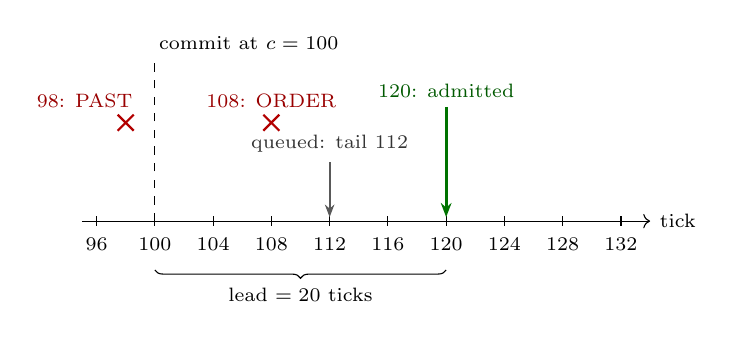
\begin{tikzpicture}[x=0.185cm,y=1cm,font=\scriptsize,
    rej/.style={draw=red!70!black, cross out, thick, minimum size=5pt, inner sep=0pt}]
  % axis, ticks 96..132
  \draw[->] (95,0) -- (134,0) node[right]{tick};
  \foreach \t in {96,100,...,132} { \draw (\t,0.06) -- (\t,-0.06) node[below=1pt]{\t}; }
  % the committing instruction
  \draw[dashed] (100,0) -- (100,2.05);
  \node[above right=0pt and -2pt] at (100,2.05) {commit at $c=100$};
  % the event already queued: the tail
  \draw[gray!70!black, thick, -{Stealth[length=1.6mm]}] (112,0.75) -- (112,0.05);
  \node[above, gray!40!black] at (112,0.75) {queued: tail 112};
  % the admitted event
  \draw[green!45!black, very thick, -{Stealth[length=1.8mm]}] (120,1.45) -- (120,0.05);
  \node[above, green!35!black] at (120,1.45) {120: admitted};
  % refused deadlines
  \node[rej] at (108,1.25) {};  \node[above=2pt, red!60!black] at (108,1.25) {108: ORDER};
  \node[rej] at (98,1.25) {};   \node[above left=2pt and -6pt, red!60!black] at (98,1.25) {98: PAST};
  % lead
  \draw[decorate, decoration={brace, mirror, amplitude=3pt}] (100,-0.62) -- (120,-0.62)
    node[midway, below=3pt]{lead $=20$ ticks};
\end{tikzpicture}
\caption{Admission. A context commits an event-creating instruction at tick $c=100$ with
one event already queued for tick 112. A deadline of 120 is strictly after both and is
admitted; it will be applied on the clock edge where the tick counter reads 120. A
deadline of 108 (before the queue's tail) or 98 (already past) is refused, and the
context stops with an ADMIT fault whose subcode names the rule.}
\label{fig:admission}
\end{figure}

The check happens at \emph{admission}, when the event enters the queue
(Fig.~\ref{fig:admission}). An event is admitted only if its deadline is strictly after
the current tick and strictly after the last event already queued, and only if it
touches pins its context owns. If any rule fails, the event is not queued, the context
stops with a fault whose subcode (PAST, ORDER, OWNER, MASK or OVERLAP) names the rule,
its pins are released, and the other three contexts carry on. A full queue is not a
fault: the instruction waits and is retried in the context's next slot. At the other end,
\emph{retirement} applies the head event on the clock edge whose tick equals its
deadline. Because admission has refused anything that could not be on time, a head event
can never be found past due. The chip still checks for that case, as the LATE\_HEAD
fault, and the proof of Section~\ref{sec:verif} shows that the check can never fire.

Every edge a program asked for therefore either happens on its tick or was refused,
visibly, before it could be late. A program that falls behind its own schedule, for
example because a computation took longer than the gap between two bits, produces a
fault at a known point instead of a stretched bit.

The deadline tests compare 32-bit values, and at the rated 50\,MHz there is no time to
compare and then drive a pin in one 20\,ns cycle. The chip therefore evaluates each test
a cycle early, for the context that commits next, and keeps the answer in a register.
This is sound because the compared values (the context's timer, its queue's tail and its
EXPECT window) change only at that context's own commit, four cycles before they are
used. The proofs assert, in every cycle that uses one of these registers, that it equals
the test evaluated on time. Decoding and operand reads are moved a stage earlier on the
same argument.

% =====================================================================================
\section{Four programs that cannot disturb one another}
\label{sec:barrel}

\begin{figure*}[t]
\centering
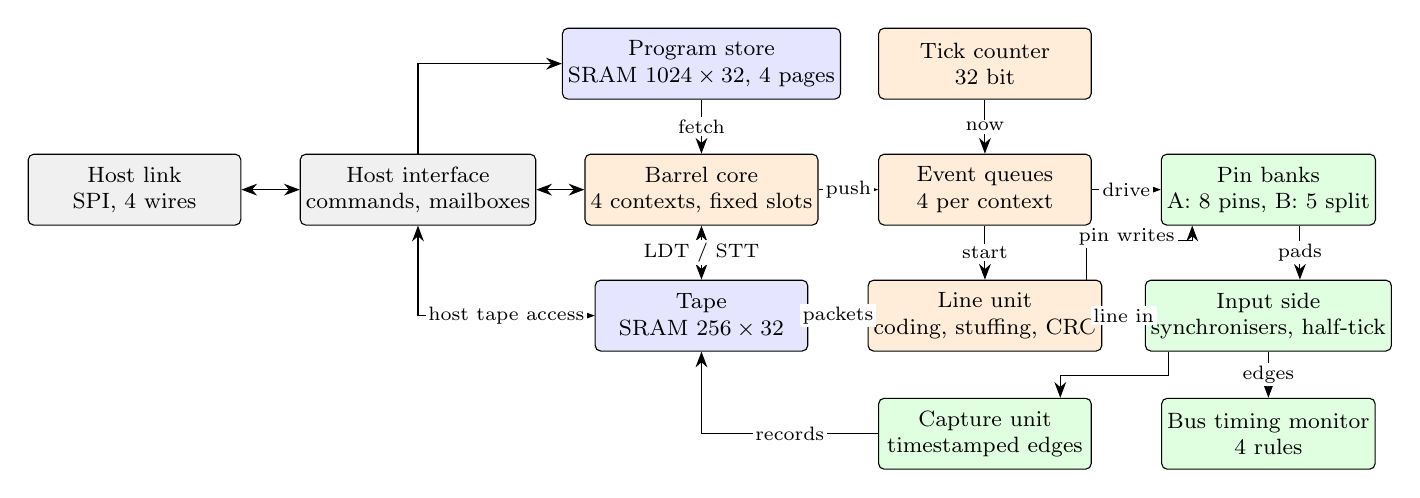
\begin{tikzpicture}[font=\footnotesize, x=1cm, y=1cm,
  blk/.style={draw, rounded corners=2pt, align=center, minimum height=9mm, minimum width=27mm,
              inner sep=2pt, fill=#1},
  blk/.default=white, ar/.style={-{Stealth[length=2mm]}},
  br/.style={{Stealth[length=2mm]}-{Stealth[length=2mm]}},
  lab/.style={font=\scriptsize, fill=white, inner sep=1pt}]
  % columns at x = 0, 3.6, 7.2, 10.8, 14.4; rows at y = 1.6, 0, -1.6, -3.0
  \node[blk=gray!12]   (host) at (0,0)      {Host link\\SPI, 4 wires};
  \node[blk=gray!12]   (hif)  at (3.6,0)    {Host interface\\commands, mailboxes};
  \node[blk=blue!10]   (imem) at (7.2,1.6)  {Program store\\SRAM $1024\times32$, 4 pages};
  \node[blk=orange!15] (core) at (7.2,0)    {Barrel core\\4 contexts, fixed slots};
  \node[blk=orange!15] (tick) at (10.8,1.6) {Tick counter\\32 bit};
  \node[blk=orange!15] (q)    at (10.8,0)   {Event queues\\4 per context};
  \node[blk=green!12]  (pins) at (14.4,0)   {Pin banks\\A: 8 pins, B: 5 split};
  \node[blk=blue!10]   (tape) at (7.2,-1.6) {Tape\\SRAM $256\times32$};
  \node[blk=orange!15] (lu)   at (10.8,-1.6){Line unit\\coding, stuffing, CRC};
  \node[blk=green!12]  (in)   at (14.4,-1.6){Input side\\synchronisers, half-tick};
  \node[blk=green!12]  (cap)  at (10.8,-3.1){Capture unit\\timestamped edges};
  \node[blk=green!12]  (mon)  at (14.4,-3.1){Bus timing monitor\\4 rules};
  % host side
  \draw[br] (host) -- (hif);
  \draw[ar] (hif.north) |- (imem.west);
  \draw[br] (hif) -- (core);
  \draw[br] (hif.south) |- node[lab, pos=0.75]{host tape access} (tape.west);
  % execution
  \draw[ar] (imem) -- node[lab]{fetch} (core);
  \draw[ar] (core) -- node[lab]{push} (q);
  \draw[ar] (tick) -- node[lab]{now} (q);
  \draw[ar] (q) -- node[lab]{drive} (pins);
  \draw[br] (core) -- node[lab]{LDT / STT} (tape);
  % line unit
  \draw[ar] (q) -- node[lab]{start} (lu);
  \draw[br] (tape) -- node[lab]{packets} (lu);
  \draw[ar] (in) -- node[lab]{line in} (lu);
  \draw[ar] ($(lu.north east)+(-2mm,0)$) -- ++(0,0.5) -| ($(pins.south west)+(4mm,0)$);
  \node[lab] at (12.6,-0.6) {pin writes};
  % input side
  \draw[ar] ($(pins.south)+(4mm,0)$) -- node[lab]{pads} ($(in.north)+(4mm,0)$);
  \draw[ar] (in) -- node[lab]{edges} (mon);
  \draw[ar] ($(in.south west)+(3mm,0)$) -- ++(0,-0.3) -| ($(cap.north east)+(-4mm,0)$);
  \draw[ar] (cap.west) -| node[lab, pos=0.25]{records} (tape.south);
\end{tikzpicture}
\caption{Architecture. Orange blocks keep time and execute, blue blocks are memories,
green blocks face the pins, grey blocks face the host. Every unit works on the one
timebase of the tick counter.}
\label{fig:arch}
\end{figure*}

The core (Fig.~\ref{fig:arch}) runs four \emph{contexts}, each with its own program
counter, four general registers, a shift register, a loop counter, a timer and an event
queue, in a fixed rotation: in cycle $t$ the context numbered $t \bmod 4$ fetches, and its
instruction commits three cycles later (Fig.~\ref{fig:barrel}). Each context issues one
instruction every four ticks whatever the others do. The barrel is there for isolation
rather than speed. A busy context cannot slow a quiet one and a waiting context leaves
its slot empty, so the instruction timing of a program can be worked out from that
program alone, and a timing certificate computed for one program still holds when four
run together. The pipeline is also simple: a context's next instruction is fetched only
after its previous one has committed, so there are no hazards, no forwarding and no
stalls.

\begin{figure}[t]
\centering
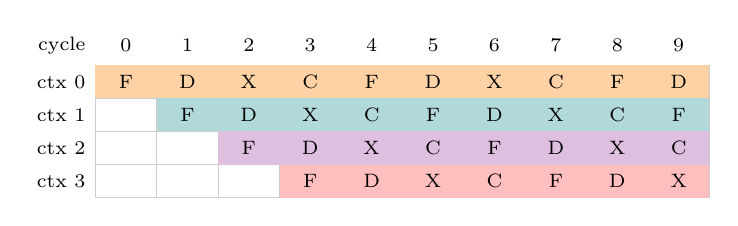
\begin{tikzpicture}[x=0.78cm,y=0.42cm,font=\scriptsize]
  \foreach \c in {0,...,9} { \node at (\c+0.5,0.6) {\c}; }
  \node[left] at (0,0.6) {cycle};
  \foreach \k in {0,...,3} {
    \node[left] at (0,-\k-0.5) {ctx \k};
    \foreach \c in {0,...,9} { \draw[gray!40] (\c,-\k) rectangle (\c+1,-\k-1); }
  }
  \foreach \k/\col in {0/orange!35,1/teal!30,2/violet!25,3/red!25} {
    \foreach \s in {0,4,8} {
      \pgfmathtruncatemacro{\f}{\s+\k}
      \foreach \st/\o in {F/0,D/1,X/2,C/3} {
        \pgfmathtruncatemacro{\cc}{\f+\o}
        \ifnum\cc<10 \fill[\col] (\cc,-\k) rectangle (\cc+1,-\k-1); \node at (\cc+0.5,-\k-0.5) {\st}; \fi
      }
    }
  }
\end{tikzpicture}
\caption{The barrel. Context $k$ fetches (F) in every cycle $t$ with $t \bmod 4 = k$; the
word is read (D), decoded beside its operand reads (X), and the instruction commits (C) at
the end of cycle $t+3$, before the context's next fetch.}
\label{fig:barrel}
\end{figure}

\textbf{Pair mode and pages.} Some protocols want more throughput from one program. When
a context's partner (context $k \oplus 2$) is switched off, pair mode lets the context
use both slots and issue every two ticks. Its next fetch is made before the previous
instruction commits, from a prediction that is checked at commit, so a wrong guess costs
an empty slot and never a wrong result. The program store holds 1{,}024 words in four
pages of 256, and each context fetches from the page its configuration names, so four
programs assembled separately can each start at address 0 with no linking step. A program
too long for one page can \emph{span} its partner's page as well, when that partner is off.

\textbf{Pins.} The 13 protocol pins form two banks. Bank A is the eight bidirectional
pins of the Tiny Tapeout pinout, each push-pull or open-drain; bank B turns the five
dedicated inputs and outputs that the host link leaves free into split pins, one input
and one output each. Instructions refer to eight logical pins and each context sees one
bank through them, so a firmware module runs on either bank unchanged and both banks can
be busy at once. Each physical pin has one owner context, and admission refuses a DRIVE
on a pin its context does not own. On an open-drain pin the value in an event is the bus
level asked for, so no register state drives an open-drain pin high, and I2C's rule that
SDA is never driven high holds by construction.

\textbf{The instruction set.} Every instruction is one 32-bit word, an 8-bit opcode and a
24-bit payload whose unused bits must be zero, so erased or uninitialised memory traps
instead of running. The 55 instructions fall into eight groups
(Table~\ref{tab:isa}). Instructions that wait, for a time, a pin pattern, a mailbox word
or a free queue entry, keep their program counter and are tried again in the context's
next slot.

\begin{table}[t]
\centering
\caption{The 55 instructions, by group}
\label{tab:isa}
\footnotesize
\begin{tabular}{@{}p{0.27\columnwidth}p{0.65\columnwidth}@{}}
\toprule
Group & Instructions \\
\midrule
Data (16) & \ins{MOV MOVI MOVHI ADD SUB AND OR XOR CMP TSTI SHL SHR ADDI CMPI LDSH STSH} \\
Control (12) & \ins{NOP HALT IRQ RET JMP JZ JNZ JC JNC DJNZ LDLC CALL} \\
Time and input (9) & \ins{RDTIME SETT ADDT WAITT ADDTR GETP WAITP GETI GETX} \\
Events (6) & \ins{EMIT EMITR EMITX EXPECT SAMPLE SEND} \\
Tape, capture (4) & \ins{LDT STT CAPT GETC} \\
Host mailboxes (4) & \ins{POP PUSH RXREADY TXREADY} \\
Line unit (2) & \ins{LINE GETL} \\
Bus monitor (2) & \ins{MON GETM} \\
\bottomrule
\end{tabular}
\end{table}

\textbf{Live reload.} The host can stop one context, rewrite its program and restart it
while the others run. A program word written during a run waits for a cycle in which the
program store has no fetch to serve, and a restarted context resumes at the frame
boundary of a run started at that point, so its certificate still holds. Whether a
reload can disturb the neighbours is a question the earlier properties do not answer;
Section~\ref{sec:verif} answers it with a non-interference proof.

% =====================================================================================
\section{Work that firmware cannot do bit by bit}
\label{sec:units}

Firmware is fast enough for most protocols but not for all of the per-bit work some of
them ask for, and a chip that knows only time would be a poor instrument. Three units do
what a program cannot do per bit, all on the same timebase and the same queue
discipline.

\textbf{The line unit.} At 24\,MHz a low-speed USB bit lasts 16 ticks, four instructions,
and in that time firmware would have to apply NRZI coding, insert a stuffed bit after six
ones and update a CRC. The line unit does that work for one owner context while the
firmware stays in charge of whole packets. A SEND event starts a packet at its deadline,
so a packet is admitted and retired like any other event. Three words on the tape
configure it: the pins, the coding, the stuffing rule, the bit period and any CRC up to
32 bits, so USB, CAN and 10BASE-T frames are configurations of one unit rather than
three blocks. When receiving, it takes its bit strobe from a recovered clock (for
UART-like, USB and CAN framing), from a cell decoder for Manchester codes (10BASE-T
\cite{ieee8023}) or from an external clock pin (to listen to an SPI bus between two other
devices). It removes stuffed bits, checks the CRC, writes the bits to the tape and
records the tick on which the packet ended. That end tick makes certified replies
possible: the firmware sets its deadline to the end of the host's packet plus a constant,
and the certificate checker proves the constant.

A 10BASE-T bit lasts 100\,ns in two halves, and at 50\,MHz one sample per tick cannot tell
an edge at a bit boundary from one in its middle once the standard's jitter is added. The
chip therefore also samples every protocol pin on the falling clock edge, the only place
it looks at a pin between ticks, and the line unit's decoder places each edge to half a
tick.

\textbf{The tape and the capture unit.} A second SRAM, the \emph{tape}, is shared by
firmware loads and stores, the line unit, the capture unit and the host, and none of
them makes another wait in a way a program can see. The capture unit writes a record of
the pin levels and the tick whenever a watched pin changes. The host can read records
during a run in the cycles the core leaves free, so a capture streams for as long as the
host keeps up, and a record is never overwritten before it has been read; a host that
falls behind ends the capture with an overflow flag, never with silently lost data. A
record has the same shape as a DRIVE event, levels and a tick, so a recorded waveform
replays tick for tick. On the Tiny Tapeout demo board, PulseView \cite{sigrok} records
from the chip through its existing logic-analyser driver.

\textbf{The bus timing monitor.} EXPECT lets a program check that another device answers
its own edges in time. The monitor checks traffic between other devices, which the chip
only watches. It holds four rules of one shape, ``the next edge of pin $B$ comes at least
MIN and at most MAX ticks after an edge of pin $A$'', which covers setup and hold times,
pulse widths, clock periods and timeouts, and it evaluates them on every tick of a run
without the program doing anything. Each rule counts its violations, and the first is
recorded with its rule, tick and measured interval. Like the line unit, the monitor has
one owner context: the first whose MON instruction commits in a run.

% =====================================================================================
\section{Verification}
\label{sec:verif}

The central claims are proved; the rest of the design is checked by methods chosen so
that each can catch what the others miss. Table~\ref{tab:verif} summarises them.

\subsection{Proofs}

The properties are written into the RTL and proved with SymbiYosys \cite{sby} on Yosys
\cite{yosys}, using ABC's property-directed reachability \cite{abc,ic3,pdr}, k-induction
\cite{kinduction} and, for one group of properties, the rIC3 model checker \cite{ric3}.
The program memory is a free input of every proof, so the proofs cover every program
anyone will load, and the tick counter may start anywhere, so the 32-bit wrap is
reachable.

\textbf{Never late.} ``No queue head is ever past its deadline'' is proved unbounded by an
assume-guarantee split \cite{assumeguarantee}. A per-context proof shows by induction
that a queue fed only with admitted events never has a late head; the core proof shows
that every event the core pushes satisfies those assumptions. The split is drawn so that
neither side assumes what the other proves. Around this property sit the others the
guarantee needs: an open-drain pin is never driven high, an unowned pin is never driven,
a faulted context drives none of its pins, a commit always belongs to the context that
owns the slot, the configuration never changes during a run, a live program write never
touches a running context's fetch, and each register that holds a decision made a cycle
early equals that decision made on time.

\textbf{Non-interference.} A miter of two copies of the core sees the same inputs on
everything a context $j$ can observe, but differs freely in every host command and
program word aimed at the other contexts. The proof, in the sense of Goguen and Meseguer
\cite{noninterference}, shows that $j$'s commits, architectural state and pins are equal
in both copies at every cycle. It is unbounded, by induction over an inductive invariant
that relates the two copies' state. The claim has a stated scope, which the host
software enforces: $j$ uses none of the shared units, since another context may own
them. The proof earned its place during development: when the bus monitor was first
added it failed, because any context could read monitor state that every other context
could shape, and the fix was to give the monitor an owner.

\textbf{The netlist is the design.} The gate-level netlist from the sign-off flow is
proved sequentially equivalent to the RTL, so the properties hold for what is fabricated
and not only for its source. The clock-gated register banks and latch banks, which have
no direct RTL counterpart, are proved equal to ordinary enabled flip-flops at every
instant, with a gated clock that cannot glitch.

\textbf{Tripwires.} Twelve of the proved properties, among them never late, open-drain
pins never driven high and unowned pins never driven, are also built into the silicon
as monitors that set a sticky flag the first time their property is seen broken. The
proofs say no flag can ever set; on real silicon, a manufacturing defect or a wrong
assumption about the environment would appear as a named, broken property rather than
as a puzzling failure.

Every proof runs in continuous integration on each change it depends on, and planted
faults show that the proofs can fail. In the final run all \NUM{PENDING-PROOF-TASKS} tasks pass: the 44 unbounded core proofs and \NUM{PENDING-PROOF-OTHER} in one job, the bounded check from reset as 52 tasks covering 72 assertion lines to depth 20 in a second, and the tripwire, line unit and non-interference proofs in a third; 15 planted bugs each make their proof fail.

\subsection{Two implementations of one specification}

The machine is defined once, cycle by cycle, in a normative specification, and
implemented twice: in the RTL, and in a Python instruction-set simulator that shares
nothing with it but the instruction encodings. The two were first written by separate
authors who could not read each other's code, so that a misreading of the specification
shows up as a disagreement rather than as two identical bugs. A co-simulation in
cocotb \cite{cocotb} on Icarus Verilog \cite{iverilog} runs both side by side and
compares every commit, every register, every pin, the queues and the memories on every
tick. In the final run it compared 191 random programs (19,850 commits; 9 more were too long for a program page) and 84 firmware cases, each against independent bus models, on both the behavioural RTL and the standard-cell build, and found no difference. The same simulator runs in the project's web page under Pyodide
\cite{pyodide}, so what a reader runs in the browser is the model the RTL is held to.

On every clock edge where something happens, the chip folds what happened into a 32-bit
\emph{execution digest}, which the simulator predicts exactly. After a run on silicon,
one read over SPI compares the whole run with the model.

\subsection{Certificates, and the chip checking them}

A static analyser, \texttt{escert}, walks every path of a firmware and proves a lower
bound on how early each event is queued before its deadline. A program whose bound is
positive can never be refused, for any input. The chip measures the same quantity while
it runs, the minimum lead of each context, so the certificate and the silicon check each
other. In the VGA Pong firmware, for example, the certificate proves that every edge of
the video signal is queued at least 1{,}597 ticks early in the sync context and 8 ticks
early in the picture context, and the simulator, the RTL, the gate-level netlist and the
FPGA all measure exactly 1{,}597 and 8. All 90 programs are certified for every input. Across the 84 co-simulated firmware cases, 84 contexts have a finite bound, and the lead measured on the RTL equals the bound in 64 of them and exceeds it in the other 20; it is never below.

\subsection{Checking the checks}

To check the tests themselves, faults are planted in the RTL one at a time across every
module and simulated on the process kit's standard-cell models \cite{mutation}; a fault
the tests do not notice is a hole in the tests. Each surviving fault is read against the
RTL and either closed with a new test, proved to change no output, or excluded with a
written argument. The final campaign planted 1,035 faults: \NUM{PENDING-MUT-KILLED} were caught by a test, \NUM{PENDING-MUT-PROVED} were proved to change no output, and \NUM{PENDING-MUT-ARGUED} are excluded with a written argument, most of them reset or start values that nothing reads before they are reloaded. None survives.

Models written from datasheets can share a misreading with the firmware they test, so
recordings of real hardware, many of them from the sigrok-dumps collection \cite{sigrok},
are used as oracles: a USB Power Delivery charger, a DS18B20 temperature sensor, an SD
card and a model railway's DCC command station among them. They found real bugs. The
UART receiver lost a byte sent straight after a stop bit by an STM32 at 460{,}800\,baud,
and the I2C EEPROM firmware, standing in for a 24LC02B, faulted at clocks below 20\,MHz;
the second showed the admission rule doing its job, since the firmware was refused, not
run with a late edge. A test that judged I2C timing from the waveform itself rather than
from the model found that the RTL and the simulator both measured monitor intervals one
tick short, a bug that lockstep comparison cannot see because the two agreed.

For every program whose protocol someone else's software can read, that software reads
the pins of the simulated run and must decode what the test asked for: sigrok's decoders
\cite{sigrok}, the IRMP infrared library, Wireshark's dissectors, the rtl\_433 receiver and
rc-switch's receiver code. They agree with 80 of the 90 programs, and each judge has a
control: the same recording with one pulse inverted must fail it. The same runs are repeated with every pin delayed by up to three
ticks each way, more than the pads and the board add, and every protocol still works.

\begin{table}[t]
\centering
\caption{Verification methods and results. Numbers are from the final
continuous-integration runs.}
\label{tab:verif}
\footnotesize
\begin{tabular}{@{}p{0.30\columnwidth}p{0.62\columnwidth}@{}}
\toprule
Method & Result \\
\midrule
Formal properties & \NUM{PENDING-PROOF-TASKS} of \NUM{PENDING-PROOF-TASKS} tasks pass, 52 of them bounded to depth 20; \NUM{PENDING-TEETH} planted bugs caught \\
Netlist vs.\ RTL & \NUM{PENDING-EQUIV} \\
Lockstep co-simulation & 191 random programs, 84 firmware cases, two builds: no difference \\
Timing certificates & 90 of 90 certified; measured lead equals the bound in 64 of 84 contexts, never below \\
Mutation testing & 1,035 faults: \NUM{PENDING-MUT-KILLED} caught, \NUM{PENDING-MUT-PROVED} proved harmless, \NUM{PENDING-MUT-ARGUED} argued, 0 surviving \\
Outside judges & decoders by others agree with 80 of 90 programs; every control fails \\
Planted firmware bugs & 823 timing bugs: 196 refuted, 23 not proven, 604 certified, 0 certified that fault \\
Slower pins & every firmware case passes with up to three ticks of delay each way \\
Test suites & 1,869 software, 12 chip (RTL and netlist), 9 through the pins \\
Held-out round & 8 of a pool of 24 drawn at random, the draw sealed: all fit; all certified and co-simulated; 6 judged by sigrok; 7 judged on the bench from captures \\
FPGA bench & 89 of 90 programs match the model and their certificates (version 3.1, 21 to 25 Nov.; version 3.2, 26 Nov.; the 14\,s chime has no bench bundle); on version 3.1, a laptop's ping over 10BASE-T; SWD on a real RP2040, judged by sigrok; a USB keyboard on a laptop; DOOM, with no word lost on the host link; a late and an unowned edge refused as \texttt{escert} predicted; a 433\,MHz remote's protocol learned from the chip's own capture, its generated receiver and transmitter run on the chip \\
\bottomrule
\end{tabular}
\end{table}

% =====================================================================================
\section{Implementation}
\label{sec:impl}

\subsection{Physical design}

The design is implemented with LibreLane \cite{librelane}, the successor of OpenLane
\cite{openlane}, on OpenROAD \cite{openroad}, for Tiny Tapeout's $8\times4$ tile slot on
IHP SG13CMOS5L \cite{ihppdk}. Table~\ref{tab:silicon} gives the result and
Fig.~\ref{fig:die} the layout, rendered from the final GDS with KLayout \cite{klayout}.

\begin{table}[t]
\centering
\caption{The signed-off layout}
\label{tab:silicon}
\footnotesize
\begin{tabular}{@{}ll@{}}
\toprule
Tiles, die & $8\times4$, $1724.16\times710.64\,\mu$m \\
Standard cells & 39{,}588, 64.4\% utilisation \\
Memories & SRAM $1024\times32$ and $256\times32$ \\
Wire & 2.38\,m \\
Clock & signed off at 20\,ns, rated 50\,MHz \\
Setup (slow, 1.08\,V, 125\,$^\circ$C) & passes down to 17.0\,ns \\
Hold slack (fast, 1.32\,V, $-40\,^\circ$C) & $+0.216$\,ns \\
Slew, capacitance & no violation at any corner \\
LVS, DRC, antenna & clean \\
\bottomrule
\end{tabular}
\end{table}

\begin{figure*}[t]
\centering
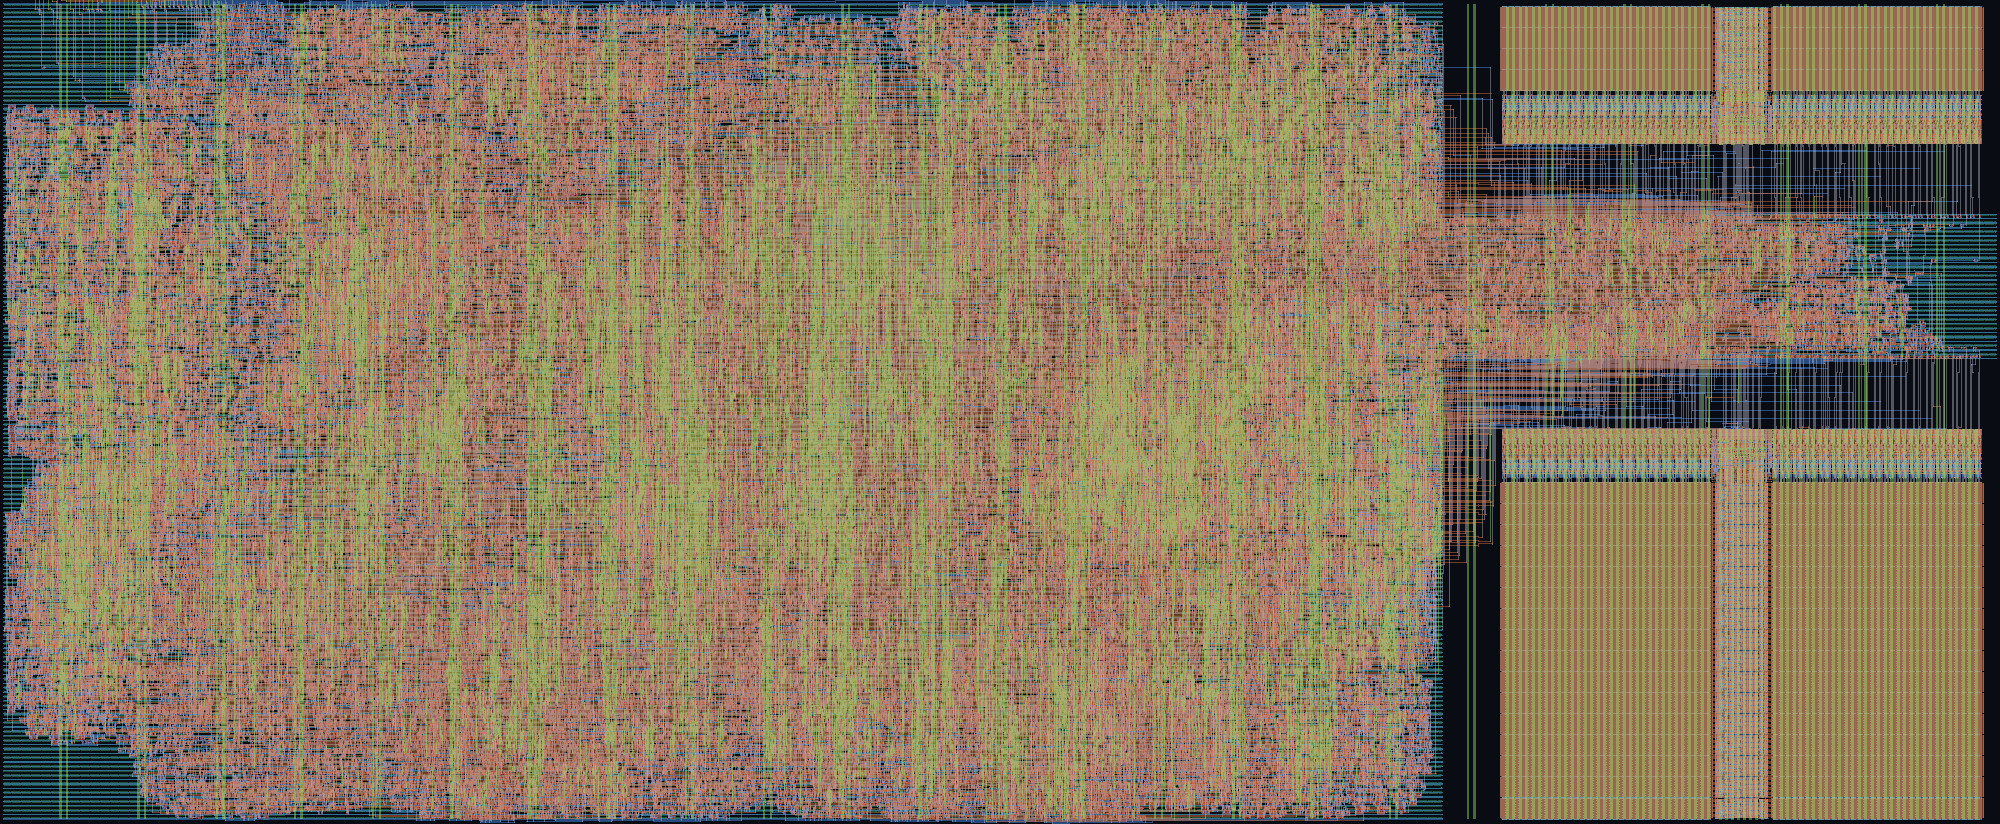
\includegraphics[width=0.66\textwidth]{fig/die.jpg}\hfill
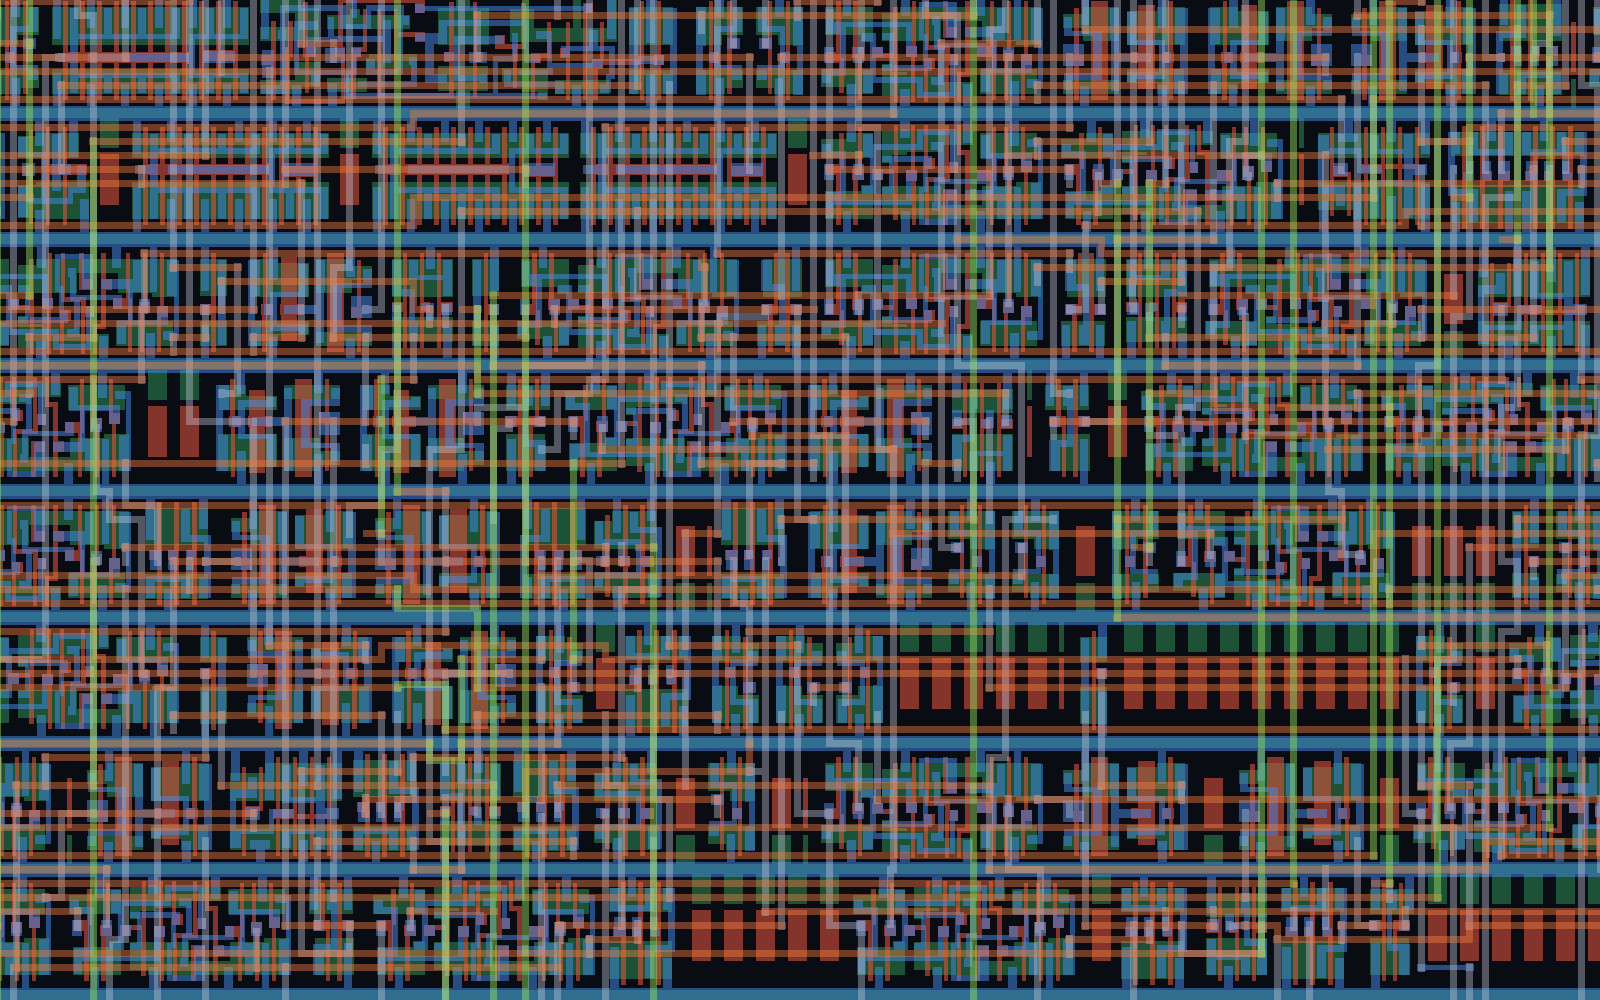
\includegraphics[width=0.32\textwidth]{fig/die_zoom.jpg}
\caption{Left: the die, $1724\times711\,\mu$m, every layer from active area to Metal4; the
program store (lower right) and the tape (upper right) share one column on the east
side. Right: a $48\times30\,\mu$m window of standard cells in the shared pipeline, with
active area (green), gate poly (red) and Metal1 to Metal4.}
\label{fig:die}
\end{figure*}

The chip is limited by wiring rather than by cell area. Only four metal layers carry
signals in a Tiny Tapeout block on this process, each SRAM blocks three of them over its
footprint, and only one of the four runs horizontally. The first $8\times4$ layouts
overflowed that layer. The final floorplan puts both memories in one column on the east
side, so the logic is a single rectangle with no macro across its horizontal paths, and
timing-driven placement keeps the core's commit logic together. Fig.~\ref{fig:blocks}
shows where each part of the design was placed.

Version 3.0 had been signed off with slew and capacitance violations left in place. Trial
hardens traced them to the repair step, which took wire capacitance at about half of what
extraction measured and judged slew only at the fast corner. With wire loads from
extraction, margins for the detours of detailed routing, a tighter slew limit for repair
and buffers before the memories' inputs, version 3.1 had no pin outside its library limits
at any corner, and version 3.2 keeps it so.

\begin{figure}[t]
\centering
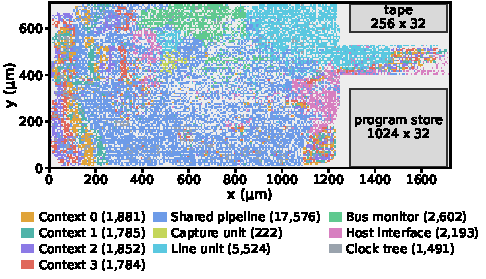
\includegraphics[width=\columnwidth]{fig/blocks.pdf}
\caption{Where the logic went: each $5\,\mu$m bin coloured by the part of the design with
the most cell area in it (cell counts in brackets). Synthesis flattens the design, so the
map is reconstructed from the net names the cells drive.}
\label{fig:blocks}
\end{figure}

Static timing analysis of the signed-off netlist with its extracted parasitics, with the
clock period shortened until setup fails, gives each corner's limit
(Table~\ref{tab:headroom}). The chip is rated at 50\,MHz because it is placed, routed and
signed off at 20\,ns; the slow corner keeps 3.0\,ns in hand, so 58\,MHz is possible but
not rated. A clock high for 40\% or 60\% of the period also passes at every corner.

\begin{table}[t]
\centering
\caption{Frequency headroom of the signed-off netlist}
\label{tab:headroom}
\footnotesize
\begin{tabular}{@{}lrrr@{}}
\toprule
Corner & Shortest period & Clock & Fails at \\
\midrule
Slow, 1.08\,V, 125\,$^\circ$C & 17.0\,ns & 58.8\,MHz & 16.9\,ns \\
Typical, 1.20\,V, 25\,$^\circ$C & 10.7\,ns & 93.5\,MHz & 10.6\,ns \\
Fast, 1.32\,V, $-40\,^\circ$C & 7.1\,ns & 140.8\,MHz & 7.0\,ns \\
\bottomrule
\end{tabular}
\end{table}

\subsection{Power}

A protocol engine spends most of its life waiting: a 115{,}200\,baud UART changes a pin
every 217 clocks at 25\,MHz. The first complete netlist did the opposite of what that
asks for. Gate-level simulation of three workloads, with the switching activity fed to
OpenSTA's power analysis, showed that a stopped chip drew 93\% of the power of a busy
one: every flip-flop saw every clock edge, and both memories read every cycle. The design
now follows one rule, pay only for work. A register that is not being written does not
see the clock (128 clock gates stand in front of almost every register), most of the large
banks are latches, 44\% smaller than flip-flops, each memory is selected only in the cycles
that read it, and a context waiting on a \texttt{WAIT} reissues its held instruction instead
of reading the program store. Table~\ref{tab:power} compares the first netlist with the
signed-off one.

\begin{table}[t]
\centering
\caption{Power at 25\,MHz, typical corner, from gate-level simulation}
\label{tab:power}
\footnotesize
\begin{tabular}{@{}lrr@{}}
\toprule
Workload & First netlist & Signed-off \\
\midrule
Sending a UART & 8.61\,mW & 1.85\,mW \\
Logic analyser capturing & 8.45\,mW & 1.54\,mW \\
Stopped & 7.99\,mW & 1.27\,mW \\
\bottomrule
\end{tabular}
\end{table}

What a stopped chip still spends is the clocked storage that must keep running and the
clock tree.

\subsection{On the bench}

\begin{figure}[t]
\centering
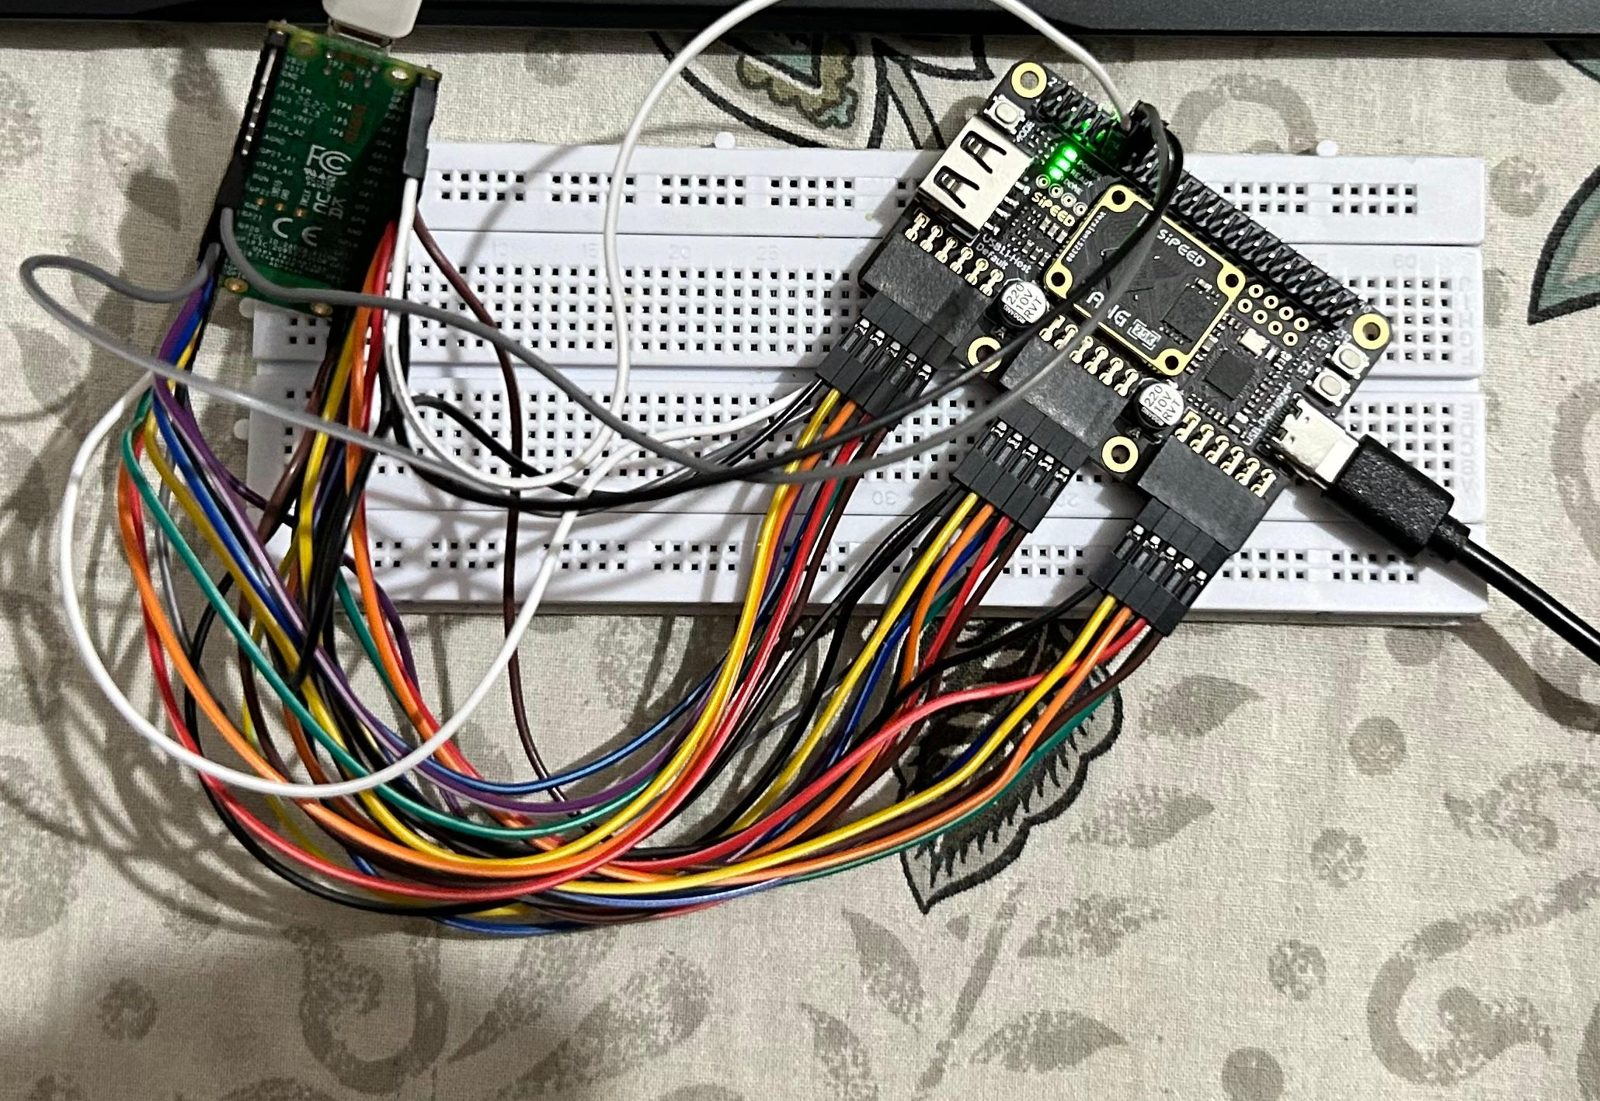
\includegraphics[width=\columnwidth]{fig/bench-setup.jpg}
\caption{The bench: a Raspberry Pi Pico W (left), playing the Tiny Tapeout demo board,
wired by 32 jumpers to a Sipeed Tang Primer 25K Dock (right), playing the chip.}
\label{fig:bench}
\end{figure}

The chip's RTL runs on an FPGA (Fig.~\ref{fig:bench}). A Sipeed Tang
Primer 25K (Gowin GW5A-25) plays the chip, built with Yosys and nextpnr \cite{nextpnr} on
Project Apicula \cite{apicula}, with plain flip-flops in place of the clock gates and latch
banks and block RAM in place of the memories. A Raspberry Pi Pico W plays the demo board
and runs the repository's bring-up script unchanged through a small shim. The script
tests the link, every memory and every pin, then loads every firmware, runs it, and
compares the chip's digest, state and measured leads with the model's prediction and the
certificate.

Version 3.2's RTL, the one hardened for silicon, runs 89 of the 90 programs through the bring-up
script (all but a 14-second chime, which has no bench bundle), and each matches the model
and stays within its timing certificate, four programs spanning two pages among them. The
build uses 15{,}251 of 23{,}040 LUTs, 5{,}262 flip-flops and 3 of 56 block RAMs, and routes
to 54.8\,MHz against the 25\,MHz it runs at, with the clock on the global network to every
one of its sinks. Earlier builds clocked the half-tick sampler's falling-edge register
through an inverter in a LUT, off the global network; the build now maps it onto the
FPGA's own falling-edge flip-flops. The same RTL also builds for an ECP5, where it routes
to 41.7\,MHz on a ULX3S 25F.

Version 3.1's bitstream, clocked at 40\,MHz, talks 10BASE-T Ethernet with a laptop. Only
resistors, capacitors and a patch cable cut open at one end connect the Dock to the
laptop's port. \texttt{eth\_tx} sent 20 of 20 test frames, which the laptop received intact.
\texttt{eth\_rx} received 20 of 20 frames of the laptop's own traffic, each with a good
frame check sequence. On the receive side an FPGA pin's input threshold stands in for the
line receiver, and the capture unit, recording the line's edges at that pin, showed how to
bias it. \texttt{eth\_trx} switches the one line unit between the two directions, which
10BASE-T's half duplex allows, and with the Pico as the IP stack it answered the laptop's
ARP request and its pings, 99 of 100 in the last run.

On the same bench the chip debugged a real RP2040 over Serial Wire Debug. Its debug port
is multi-drop (SWD protocol version~2): two cores and a rescue port share the wires, start
dormant, and answer only once woken and selected, which \texttt{swd\_idcode} now does. The
chip read the port's ID, the AHB-AP's ID and a boot ROM word from either core. A
third-party logic analyser firmware, running on the target Pico beside its debug port,
recorded the wires, and sigrok's \texttt{swd} decoder read all 15 accesses after the
wake-up exactly as the chip reported them, with every SWCLK phase at the 640\,ns the
firmware is built for; the control, one SWDIO pulse inverted, fails.

The chip has no USB hardware either. With its two data pins wired to a laptop's USB port
through two 27\,$\Omega$ resistors, and a 1.5\,k$\Omega$ pull-up that the Pico switches on
once the firmware runs, \texttt{usb\_hid} enumerated as a low-speed keyboard, Windows read
its descriptors and product string, and the chip typed the line it was given into a
window, up to 151 characters, exactly, in six runs out of six. Each line carried a number
drawn on the laptop for that run, so only a working keyboard could have typed it.

The refusal that the chip is built around has also run on these pins. Two programs ask for
the impossible: a UART whose bit is five ticks long, so its second edge cannot be queued
before its deadline, and a drive on a pin its context does not own. \texttt{escert} refutes
both before they run. On the bench each faulted at the instruction and tick the model
predicts (ADMIT with subcode PAST at tick~35, and OWNER at tick~15), with the model's
digest. While each run was still on, the Pico swapped its pull-ups on the program's pins
for pull-downs and read them all low, so the faulted context had let go of its pin and the
unowned one was never driven, and the chip's proof tripwires, its own monitors for a late
FIFO head, an unowned drive and a faulted context driving, read zero.

Learning ran on the chip's own capture. The Pico played the frames of a PT2262 433\,MHz
socket remote, from a sigrok recording, onto one pin, and the capture unit recorded their
200 edges. From that capture \texttt{esclearn} recovered the code (25 bits a frame, a
290\,$\mu$s or 920\,$\mu$s mark per bit) and all four of the remote's words, and
\texttt{escgen} generated a receiver and a transmitter, both certified. On the chip the
receiver read 8 of 8 frames as their words, and the transmitter sent an address the remote
never had, which the learned model read back from the Pico's timing of the pin.

% =====================================================================================
\section{What it does}
\label{sec:apps}

Ninety programs run on the chip, eight of them from the held-out round at the end of this
section. Among them are UART, SPI, I2C, CAN, PS/2, WS2812, 1-Wire, JTAG, ARM SWD, DMX512,
HDMI-CEC, DALI, SENT, DShot, low-speed USB and 10BASE-T Ethernet; none of these protocols
is in the hardware. The examples below show the reach of the mechanisms, and the held-out
round tests it.

\textbf{A USB keyboard.} A 187-instruction firmware enumerates on a real Linux kernel
through USB/IP \cite{usbip}, with the simulated chip at the other end, and on a laptop's
USB port with the FPGA build of the chip. The certificate
checker proves that every reply leaves exactly 72 ticks after the end of the host's
packet, which is 75 ticks or 4.69 bit times at the pins, inside the 2 to 6.5 bit times USB
allows \cite{usb20}.

\textbf{Record it, speak it.} Pointed at a transmitter it has never seen, such as an
infrared remote, the chip records the waveform, a host tool works out the protocol's
timing table from the recording, a generator turns the table into firmware that
\texttt{escert} certifies, and the chip then sends new messages in that protocol. The same
table also gives a receiver, which reads the remote's frames back, those never recorded
included. A recording that fits no model is refused with the reason.

\begin{figure}[t]
\centering
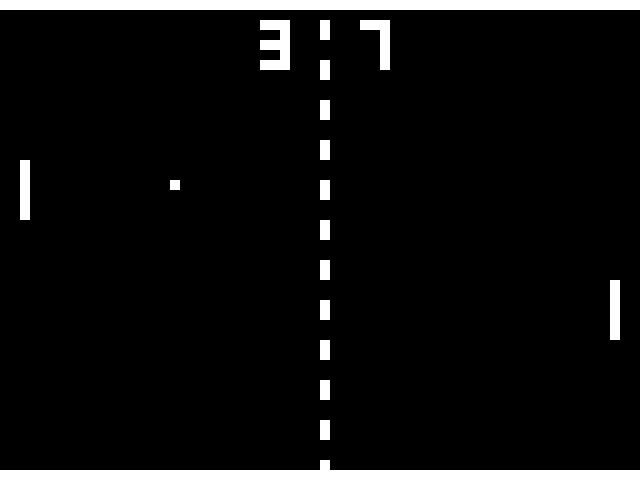
\includegraphics[width=0.48\columnwidth]{fig/vga-pong.png}\hfill
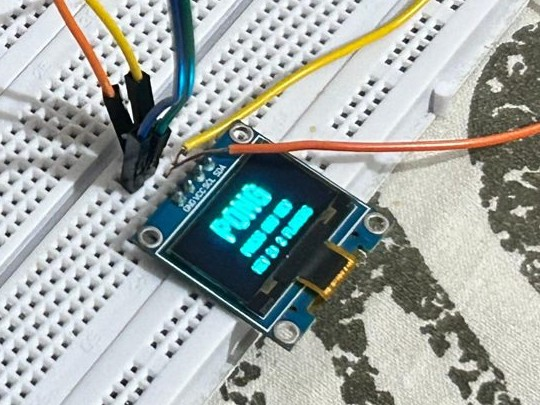
\includegraphics[width=0.48\columnwidth]{fig/oled-crop.jpg}
\caption{Left: a frame of VGA Pong, $640\times480$ at 60\,Hz from five bank~B pins.
Right: the four-context OLED Pong on the FPGA bench, showing its title screen.}
\label{fig:pong}
\end{figure}

\textbf{Pong, on two screens.} Two contexts drive a VGA monitor at $640\times480$ and
60\,Hz from five bank B pins (Fig.~\ref{fig:pong}): one makes the syncs, the other draws a
framebuffer from the tape and runs the game in the vertical blank. Every edge of the
picture has a deadline fixed in advance and only the colours come from data, so the
certificate proves that no edge is late. On the FPGA bench the same game runs on an
SSD1306 OLED as four programs, one per context and page: a display driver that speaks I2C,
a text layer, the game and a menu. They communicate only through queues on the tape, and
every I2C edge stays certified.

\begin{figure}[t]
\centering
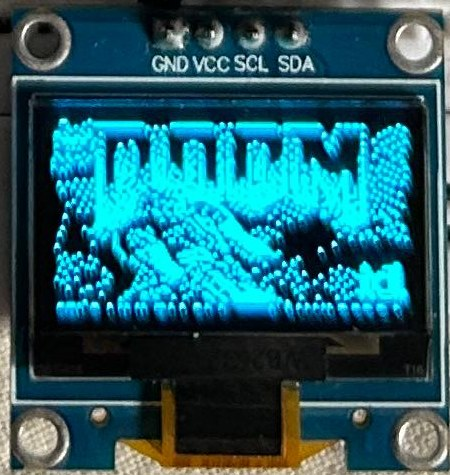
\includegraphics[width=0.55\columnwidth]{fig/doom-crop.jpg}
\caption{DOOM's title screen on the SSD1306, sent by the chip's RTL on the FPGA bench while
a Pico W runs the game.}
\label{fig:doom}
\end{figure}

\textbf{DOOM, with the chip as its input/output processor.} A Raspberry Pi Pico W runs the
shareware DOOM \cite{rp2040doom} and hands every frame and every sound to the chip as words
on the host link (Fig.~\ref{fig:doom}). One context streams each frame, averaged from
$320\times200$ to $128\times64$ and dithered, to the OLED over I2C; a second plays the
sound as pulse-width modulation, 8-bit samples at 11{,}025 a second on an 88\,kHz carrier,
into a laptop's headset jack through a low-pass filter; a third checks the I2C bus against
Fast-mode limits; and a fourth can record the sound pin. The game sets its own pace and the
protocols set theirs. A mailbox holds two words and STATUS shows only whether it is full,
so the host pushes at most one word per context per STATUS read, which makes the link
lossless by construction: in a three-minute run on the bench, 523{,}797 words went over it
and none was lost. Two pieces of firmware were added for it with no hardware change: the
PWM sound program, with every edge certified, and a stream mode that lets the I2C writer
send a frame from the mailbox while the host renders the next. A late word only holds SCL
low, which I2C allows.

\textbf{Protocols without new hardware.} Version 3's hardware was complete on 14 November.
Since then the OLED Pong, an I2C burst writer and nine more protocols have been added,
from an XY2-100 laser-scanner link in four cooperating contexts
to a FlexRay frame with both of its CRCs computed on the chip. Version 3.1's one new
capability, span, came for a Modbus device with its whole data model, and every earlier
program runs on it unchanged.

\textbf{Protocols it was not designed for.} Every program above is for a protocol someone
chose knowing what the chip could do. The held-out round takes that choice away. On 4 November a pool of 24 protocols was fixed, each with a public specification
and none in the firmware; eight were drawn from it at random, and the SHA-256 of the drawn
list, with a 256-bit salt, was committed before any was written. The eight were written on
24 November on version 3.1, with the chip, assembler and simulator as tagged: a
MIL-STD-1553B remote terminal, an S/PDIF transmitter, a Microwire EEPROM master, a DHT22
host, a BiSS C encoder master, a PS/2 host, a SNES pad reader and an M-Bus slave. Each was
tested against a bus model written by a separate session from the specification and an
interface it was given, and barred from the firmware and its tests, with planted
variants that must fail, then certified, co-simulated on the RTL, read by sigrok where it
has a decoder (six of eight) and run on the FPGA bench, where seven were judged from a logic
analyser's capture; the 1553B terminal makes no edge without a bus controller.

All eight fit, each with stated limits, and no instruction was missing: the timed events
placed every edge where its specification puts it. What ran short was registers and
program words, not timing. Three programs span two pages, and where a bit is only a few
instructions the protocol sets a floor on the clock, 40\,MHz for the 1553B terminal. The
round found no bug in the chip. It found one in \texttt{escert}, which had never checked
that a line-unit configuration is valid and drives only pins its context owns, and now
does. The pool itself was chosen, and has been public while the hardware went on changing, so the
round shows that the chip takes protocols nobody picked to fit it, not that it takes any
protocol. The draw, the seal and every result are published with the design.

% =====================================================================================
\section{How it got here}
\label{sec:history}

The first design started from a question different from the obvious one. Instead of how
fast the chip can toggle a pin, it asked how the chip can know, at the moment a program
asks for an edge, whether that edge will be on time. An early proposal wrapped that idea
in much more, including weighted scheduling between programs and timing claims resting
on cell counts nobody had measured; a review found that its pieces did not fit together,
and nearly everything but timestamped I/O was cut. The rebaseline that followed set the
shape the chip still has: a program store in SRAM (a $256\times32$ macro takes about
$50{,}000\,\mu$m$^2$, against roughly $700{,}000\,\mu$m$^2$ for the same storage in
flip-flops), the fixed four-slot barrel, input checks in the same deadline queue as
outputs, chip-measured scheduling margin, open-drain level semantics and a single clock
domain. A clock's escapement releases exactly one tick at a time, which is what
admission does; that gave the name.

The specification and its two implementations (Section~\ref{sec:verif}) came before any
layout. By the time the first layout existed, the two
agreed tick for tick on every firmware and on a thousand random programs, and admission
had already refused four firmware bugs that a conventional processor would have run with
a late edge. Each later version added one capability while keeping every older program's
behaviour, digest included (Table~\ref{tab:history}).

\begin{table}[t]
\centering
\caption{Versions and their layouts}
\label{tab:history}
\footnotesize
\begin{tabular}{@{}lp{0.52\columnwidth}rr@{}}
\toprule
Ver. & Added & Cells & Util. \\
\midrule
1.0 & four contexts, events, admission & 28{,}749 & 55.6\% \\
1.1 & tape, capture, digest, clock gating & 23{,}978 & 55.2\% \\
1.2 & pin bank B (8 to 18 signals) & 25{,}864 & 58.9\% \\
1.3 & streaming capture & 25{,}931 & 59.7\% \\
1.4 & line unit; latch banks & 27{,}972 & 58.2\% \\
1.5 & deadline tests a cycle early & 28{,}961 & 59.5\% \\
1.6 & early decode and operands; 20\,ns & 32{,}239 & 65.9\% \\
1.7 & pair mode, live reload & 32{,}147$^*$ & 66.0\%$^*$ \\
2 & pages, tripwires; $8\times4$ & 34{,}222$^*$ & 58.6\%$^*$ \\
3 & receive strobes, half-tick sampler, monitor & 37{,}230 & 61.9\% \\
3.1 & span, reset synchroniser, electrical rules & 38{,}514 & 62.6\% \\
3.2 & registers clocked only when written; parked waits & 39{,}588 & 64.4\% \\
\bottomrule
\end{tabular}

\vspace{2pt}\raggedright\scriptsize Versions 1.0 to 1.7 are $6\times4$ tiles.
$^*$Versions 1.7 and 2 were not released; their features are part of version 3. Their
figures are trial layouts: version 1.7's with pair mode only, before live reload, and
version 2's the one its release campaign froze.
\end{table}

Speed came late. Version 1.4 met timing only to 28.6\,MHz at the slow corner, and its
longest paths all had one shape: a 32-bit comparison of a deadline with the tick counter
followed by a pin update in the same cycle. Version 1.5 moved the comparisons a cycle
earlier and reached 38.6\,MHz; version 1.6 moved decode and operand reads too and was
signed off at 20\,ns. The move to $8\times4$ tiles brought the project's most useful
physical finding, that the larger die did not make routing easier (Section~\ref{sec:impl}),
and the floorplan that answered it closed with margin at 20\,ns. The last
round of hardware work turned the chip's exactness outward, with the receive side of the
line unit, the half-tick sampler and the bus timing monitor. Version 3.1 added span for a
Modbus device that needed more than one page, released the reset through a synchroniser,
and corrected the layout's repair until every electrical rule was met. Version 3.2 was for
power alone: its clock gating and parked waits took a stopped chip from 3.36 to 1.27\,mW
with nothing a program sees changed.

% =====================================================================================
\section{Limits}
\label{sec:limits}

The guarantee is about the chip's own edges. Its inputs pass through two-flop
synchronisers, so an input change reaches the logic two ticks after the clock edge that
samples it, and a pulse shorter than a tick may not be seen at all, as on any synchronous
design; because every input sees the same delay, intervals between input edges are still
measured correctly. The non-interference result holds within its stated scope, for a
context that uses none of the shared units. Certificates cover the programs they were
computed for, and a program without one is still never late, only possibly refused. The
FPGA bench tests the design, its firmware and its host interface on real pins, not the
silicon: the hardened netlist, the clock gates and latch banks and the SRAM macros are
covered by the gate-level suites, the equivalence proofs and timing sign-off instead.
The Tiny Tapeout multiplexer and pads add delays outside the design, which limit what a
board can use rather than what the chip guarantees inside its tiles.

% =====================================================================================
\section{Conclusion}

In Escapement, every pin change is an
event with an absolute deadline, checked when it is queued and either applied on its
tick or refused, and that property is proved for every program on RTL equivalent to the
netlist sent to fabrication. The fixed-slot barrel makes a program's timing its own, so
static certificates compose and the chip can measure the margin they predict. On that
base, protocols are programs: ninety of them, eight drawn at random from a sealed list,
run on a 130\,nm design that fits in
$8\times4$ Tiny Tapeout tiles and uses 1.85\,mW to send a UART. Everything described here,
RTL, firmware, tools, proofs and the flow configuration, is open source.

\section*{Acknowledgment}

I thank the Tiny Tapeout project and IHP, whose shuttle and open process kit make
fabrication possible; the developers of LibreLane, OpenROAD and Yosys, whose tools carried
the design to a layout and through its proofs; and the contributors to sigrok-dumps, whose
recordings of real hardware let the chip be judged against it.

\bibliographystyle{IEEEtran}
\bibliography{refs}

\end{document}
